\section{Généralités}

\subsection{Restriction du modèle}

La figure~\ref{modele_restreint} met en évidence le sous ensemble que nous avons choisi d'étudier, qui a été déterminé à partir des contraintes énumérées au chapitre~\ref{chapter:les_contraintes}. Cette sous partie correspond à ce que Laborit nomme le néocortex.

\begin{figure}[H] 
\includegraphics[width=\textwidth]{files/modele_restreint} 
\caption{Modèle restreint déterminé à partir des contraintes énumérée au chapitre~\ref{chapter:les_contraintes}} 
\label{modele_restreint}
\end{figure}

\subsection{Architecture générale}

L'architecture générale de notre modèle est présenté sur la figure ~\ref{schema_general}. L'IA est composé de trois modules :
\begin{itemize}
\item l'analyseur, composé d'un \emph{RuleBook}, d'un analyseur conceptuel de base et d'un analyseur conceptuel poussé,
\item le raisonneur, qui contient un moteur de choix, et un module d'introspection,
\item et la mémoire, structurée avec une interface nommée mémoire primaire.
\end{itemize}

\begin{figure}[H] 
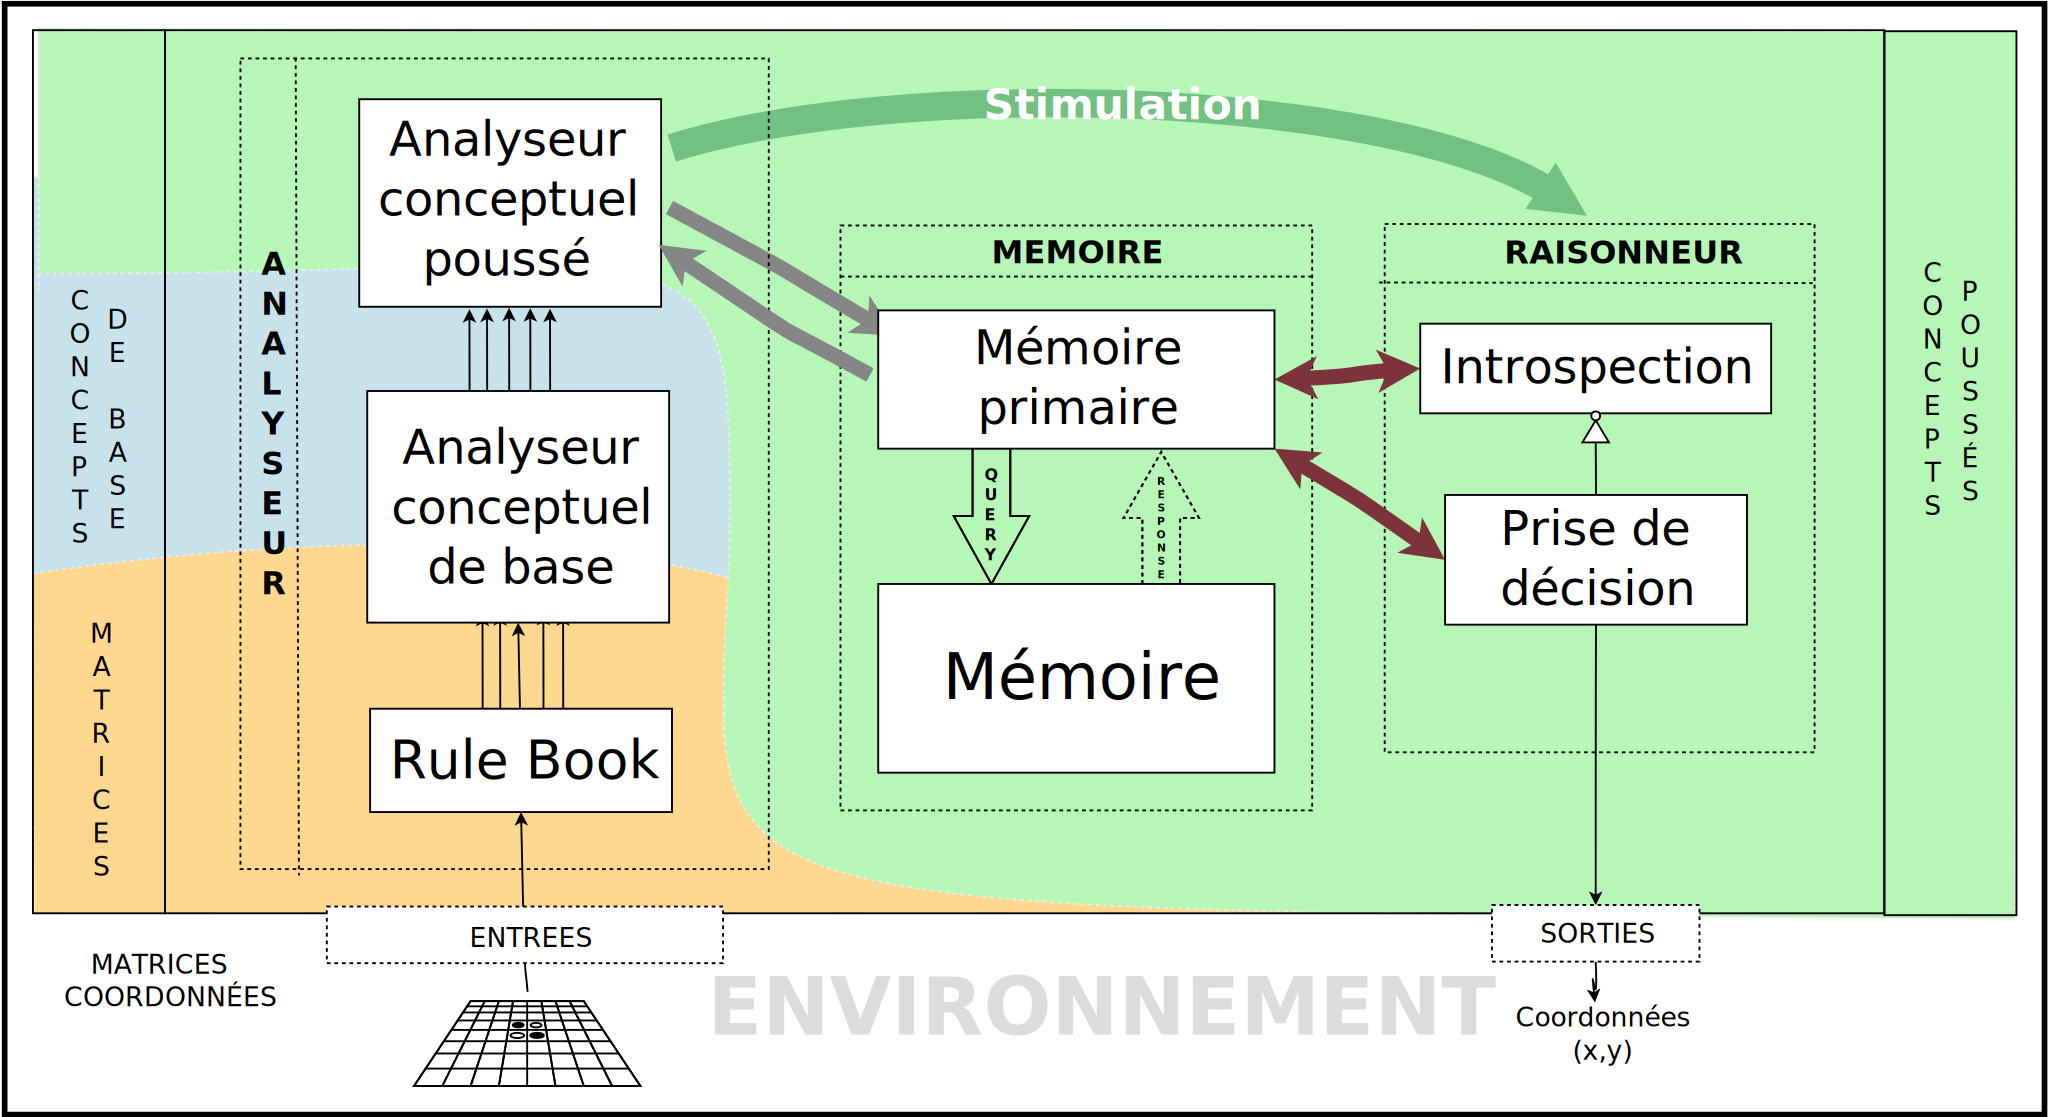
\includegraphics[width=\textwidth]{files/simplified_general_diagram} 
\caption{Schéma général} 
\label{schema_general}
\end{figure}

L'environnement est externe à l'agent, et interagit avec ce dernier via ses entées~/~sorties.

Trois niveaux de données sont manipulés par l'IA :
\begin{itemize}
\item les informations basiques, sous la forme de matrices, provenant de l'environnement,
\item un premier niveau correspondant aux concepts primaires,
\item ainsi que les concepts poussés, qui sont stockés en mémoire et qui permettent de raisonner.
\end{itemize}

\subsection{Déroulement d'un coup}

La figure~\ref{diag_sequence_coup} (page~\pageref{diag_sequence_coup}) décrit les interactions entres les modules de l'IA lorsque qu'un nouveau coup doit être joué.

Un plateau, décrit sous forme matricielle, est transmit par l'environnement (et via un module d'\emph{E/S}\footnote{Entrée/Sortie}) au \emph{RuleBook}. Ce dernier détermine l'ensemble des coups possibles et transmet à l'\emph{ACB}\footnote{Analyseur Conceptuel de Base} une série de matrices correspondantes à l'état du plateau après chaque coup joué. Ce module traduit les matrices en un formalisme logique. On obtient alors des concepts poussés qui sont fournis à l'\emph{ACP}\footnote{Analyseur Conceptuel Poussé}. Ce dernier interroge la mémoire pour obtenir une série de formes remarquables. L'\emph{ACP} complète chaque concept poussé en y associant l'ensemble des formes qui sont présentes dans l'état du plateau. Une fois analysés, ces concepts poussés sont stockés en mémoire primaire. L'\emph{ACP} stimule ensuite le moteur de choix qui, après avoir inhibé le moteur d'introspection, accède aux concepts stockés en mémoire primaire et fait un choix. Cette décision est successivement transmise au module d'\emph{E/S} puis à l'environnement.

\begin{figure}[p]
\centering
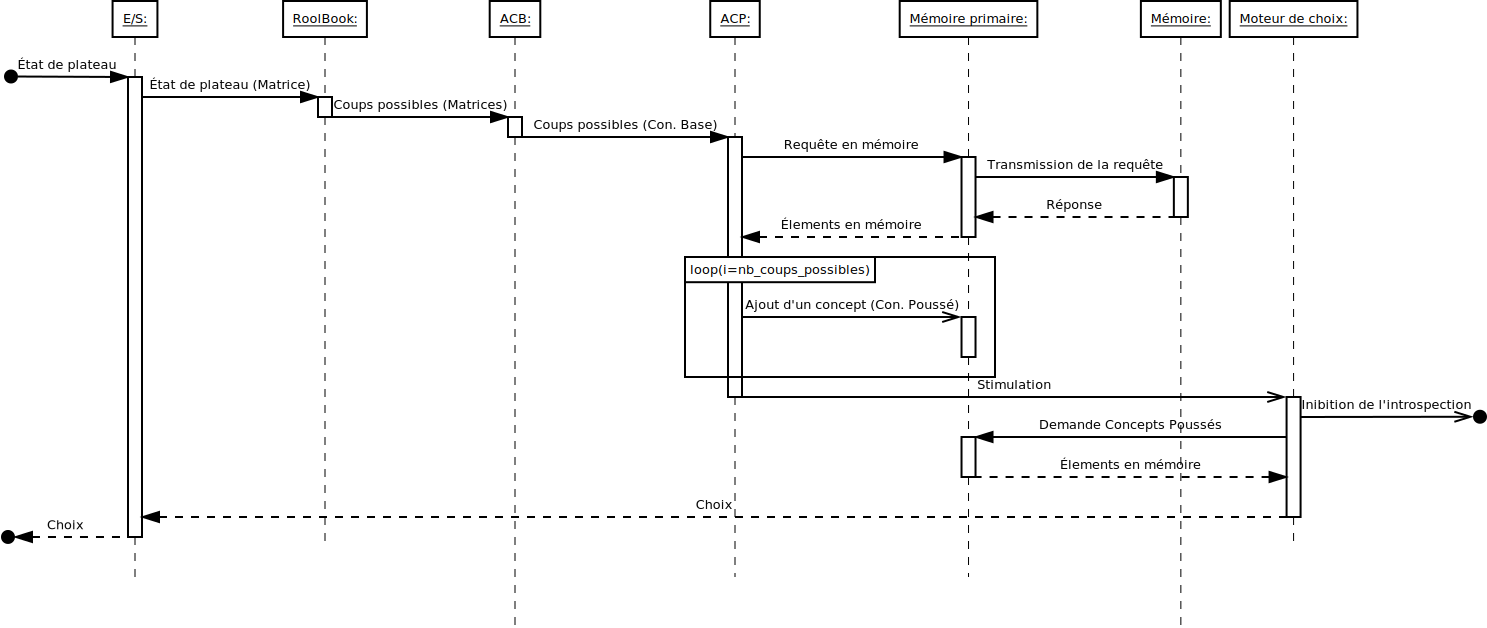
\includegraphics[width=0.9\textheight,angle=90]{files/analyse/sequence}
\caption{Diagramme de séquence sommaire de déroulement d'un coup.}
\label{diag_sequence_coup}
\end{figure}
